\documentclass[11pt]{article}
\usepackage{amsmath,amssymb,amsthm}
\usepackage{graphicx}
\usepackage[margin=1in]{geometry}
\usepackage{enumitem}

\theoremstyle{remark}
\newtheorem{remark}{Remark}
\newtheorem{caveat}{Caveat}

% Reference-textbook convention (Stage 5a): Goldstein, Poole \& Safko,
% "Classical Mechanics," 3rd ed. governs notation, equation formatting/
% numbering, and physical conventions (Gaussian units, sigma(Omega) for the
% differential cross section, the H = sum p_i qdot_i - L sign convention).
% The lecture's own structural/pedagogical devices (numbered Remarks, the
% CAVEAT aside, the crossed-out MIDTERM REMARK) are preserved as their own
% blocks rather than dissolved into continuous textbook prose, per the
% Stage 5a review panel's scoping of the convention.

\title{Scattering by a Central Potential;\\ The Hamiltonian and Hamilton's Equations of Motion}
\author{HC 6001 --- Dr.\ Castillo}
\date{October 22, 2024}

\begin{document}
\maketitle

\noindent This chapter typesets the instructor's handwritten lecture notes
for HC~6001 (October 22, 2024) in the notation and equation conventions of
Goldstein, Poole \& Safko, \emph{Classical Mechanics}, 3rd~ed. Two topics are
covered: the kinematics and dynamics of scattering by a central potential,
culminating in the Rutherford cross section (Sections~1--3), and the passage
from the Lagrangian to the Hamiltonian formalism via the Legendre transform,
the opening of the course's Chapter~8 (Section~4). Occasional remarks below
that refer to ``the original notes'' point to the instructor's handwritten
source pages, reproduced in part as figures throughout.

\section{Kinematics of Scattering by a Central Potential}

Consider a particle of mass $m$ incident on a fixed central-potential scattering
center with energy $E$, velocity $v_0$, and angular momentum $\ell$:
\begin{align}
  E &= \tfrac{m}{2} v_0^2, &
  v_0 &= \sqrt{2E/m}, &
  \ell &= s m v_0 = s\sqrt{2mE},
\end{align}
where $s$ is the \emph{impact parameter}. Equivalently, $s = \ell/\sqrt{2mE}$.

\begin{figure}[h]
  \centering
  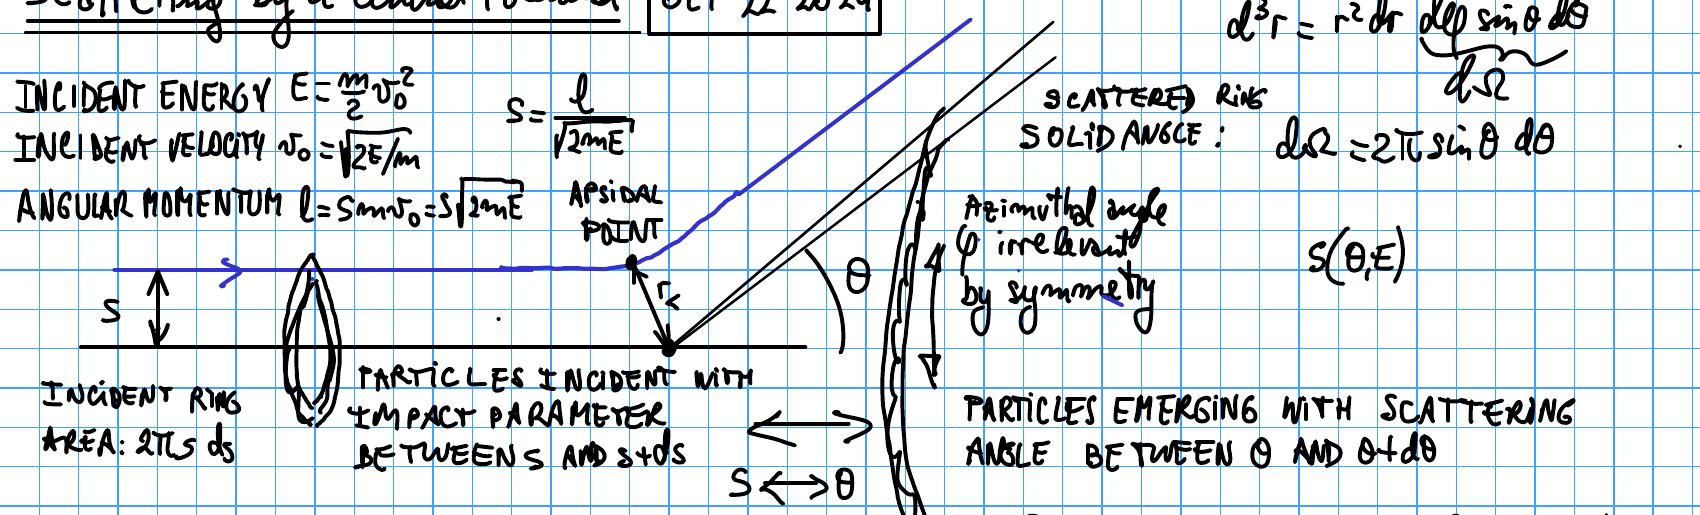
\includegraphics[width=0.95\textwidth]{figures/fig_impact_ring.png}
  \caption{Impact-parameter and scattered-ring geometry: particles incident
  with impact parameter between $s$ and $s+ds$ (left) emerge with scattering
  angle between $\theta$ and $\theta+d\theta$ into the ring of solid angle
  $d\Omega$ (right). The azimuthal angle $\varphi$ is irrelevant by the
  symmetry of a central potential, so the scattering problem reduces to a
  function $s = S(\theta,E)$.}
  \label{fig:impact-ring}
\end{figure}

As Fig.~\ref{fig:impact-ring} also records, the solid-angle element used
throughout is $d^3r = r^2\,dr\,d\varphi\sin\theta\,d\theta$, with
$d\Omega \equiv d\varphi\sin\theta\,d\theta$ integrated over $\varphi$ to give
$d\Omega = 2\pi\sin\theta\,d\theta$ below.

The incident intensity is the number of particles incident per unit time per
unit cross-sectional area of the beam,
\[
  I = \frac{\#\ \text{particles incident per unit time}}{\text{incident beam cross-section area}}.
\]
An incident ring of area $2\pi s\,ds$ carries particles with impact parameter
between $s$ and $s+ds$; by conservation of particle number these emerge into
the solid angle $d\Omega = 2\pi\sin\theta\,d\theta$ subtending the corresponding
range of scattering angle:
\[
  I(2\pi s)\,|ds| \;=\; I\,\sigma(\theta)\,2\pi\sin\theta\,|d\theta|,
\]
where $\sigma(\Omega)\,d\Omega$ is, by definition, the number of particles
scattered into $d\Omega$ per unit time, divided by $I$. Hence
\begin{equation}
  \boxed{\sigma(\theta) = \frac{s}{\sin\theta}\left|\frac{ds}{d\theta}\right|},
  \qquad
  \boxed{\sigma_T = \int d\Omega\,\sigma(\Omega)},
  \label{eq:sigma-def}
\end{equation}
the \emph{differential} and \emph{total} scattering cross sections.

\section{Relation Between Impact Parameter and Scattering Angle}

Let $\psi$ be the angle, measured at the apsidal point, between the incoming
asymptote and the line to the center of force. Two cases arise, depending on
whether the force is repulsive or attractive:

\begin{figure}[h]
  \centering
  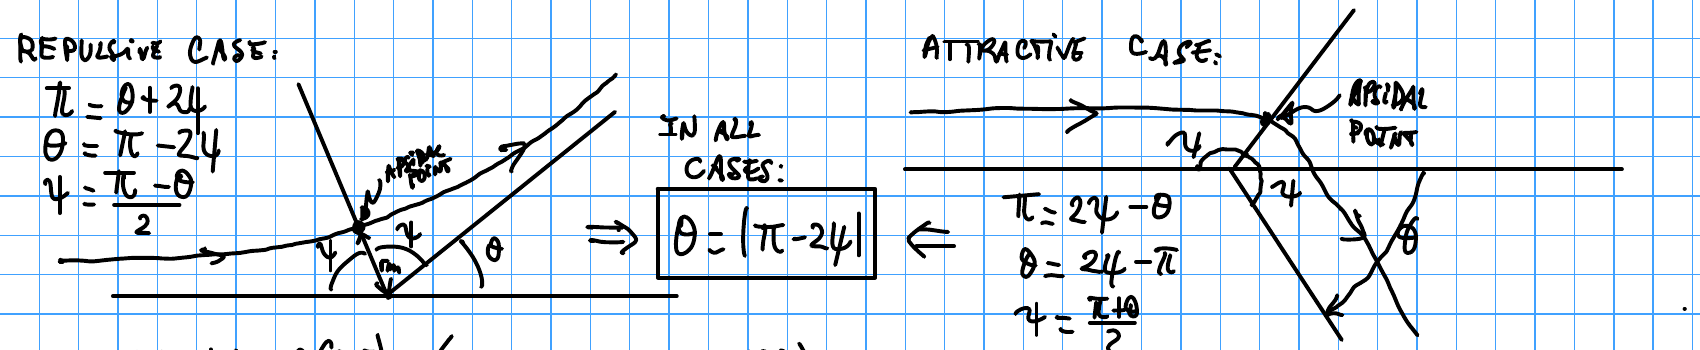
\includegraphics[width=0.95\textwidth]{figures/fig_scatter_cases.png}
  \caption{Repulsive case ($\pi = \theta + 2\psi$, left) and attractive case
  ($\pi = 2\psi - \theta$, right); $\psi$ is the angle at the apsidal point
  between the incoming asymptote and the line to the force center.}
  \label{fig:scatter-cases}
\end{figure}

\begin{align}
  \text{Repulsive:}\quad \pi &= \theta + 2\psi, & \theta &= \pi - 2\psi, & \psi &= \frac{\pi-\theta}{2}; \\
  \text{Attractive:}\quad \pi &= 2\psi - \theta, & \theta &= 2\psi - \pi, & \psi &= \frac{\pi+\theta}{2}.
\end{align}
In both cases,
\begin{equation}
  \boxed{\theta = |\pi - 2\psi|}.
  \label{eq:theta-psi}
\end{equation}

For a general central potential $V(r)$, conservation of energy and angular
momentum give
\[
  E = \frac{m}{2}\dot r^2 + V(r) + \frac{\ell^2}{2mr^2}, \qquad
  \dot r = \left[\frac{2}{m}\Big(E - V(r) - \frac{\ell^2}{2mr^2}\Big)\right]^{1/2},
\]
and, with $\ell = mr^2\dot\theta$,
\[
  d\theta = \dot\theta\,dt = \frac{\ell}{mr^2}\,\frac{dr}{\dot r}
  = \frac{s\,r^{-2}\,dr}{\left[1 - \dfrac{V(r)}{E} - \dfrac{s^2}{r^2}\right]^{1/2}},
\]
using $\ell/\sqrt{2mE} = s$. Integrating from the apsidal distance $r_m$ (where
$u_m \equiv 1/r_m$) out to $r\to\infty$, and substituting $u=1/r$,
\begin{equation}
  \psi = \int_0^{u_m} \frac{s\,du}{\left[1 - \dfrac{V(1/u)}{E} - s^2u^2\right]^{1/2}},
\end{equation}
so that, combined with Eq.~\eqref{eq:theta-psi},
\begin{equation}
  \boxed{\theta(s) = \left|\,\pi - 2\int_0^{u_m} \frac{s\,du}{\left[1-\dfrac{V(1/u)}{E}-s^2u^2\right]^{1/2}}\,\right|}.
  \label{eq:universal-theta}
\end{equation}
From $\theta(s)$ one computes $|ds/d\theta| = 1/|d\theta/ds|$ and hence
$\sigma(\theta)$ via Eq.~\eqref{eq:sigma-def}.

\begin{remark}
Equations \eqref{eq:theta-psi}--\eqref{eq:universal-theta} are valid for
\emph{any} central potential $V(r)$; nothing in this section has assumed a
specific force law.
\end{remark}

\section{Coulomb (Rutherford) Scattering}

We now specialize the universal result Eq.~\eqref{eq:universal-theta} to the
Coulomb interaction between two charges $Ze$ and $Z'e$ (Gaussian units,
following Goldstein's convention), with force $f = ZZ'e^2/r^2 = -k/r^2$ and
potential $V(r) = -k/r$, $k = -ZZ'e^2$.

For $V(r) = -k/r$ the orbit is a conic section,
\begin{equation}
  \frac{1}{r} = C_1\big[1 + \varepsilon\cos(\tilde\theta - \tilde\theta')\big],
  \qquad C_1 = \frac{mk}{\ell^2}, \qquad
  \varepsilon = \left[1 + \frac{2E\ell^2}{mk^2}\right]^{1/2}
             = \left[1 + \left(\frac{2sE}{ZZ'e^2}\right)^{2}\right]^{1/2} > 1
  \label{eq:orbit}
\end{equation}
for $E>0$, using $\ell = s\sqrt{2mE}$.

\begin{remark}[Orbit classification]
For this potential the sign of $E$ fixes the orbit type: $E>0$ gives a
hyperbolic orbit ($\varepsilon>1$), $E=0$ a parabolic orbit ($\varepsilon=1$),
and $E<0$ an elliptic orbit ($\varepsilon<1$). This three-way classification
by the sign of $E$ is specific to $V(r)=-k/r$ and does not hold for a general
central potential. Scattering states have $E>0$, so only the hyperbolic case
is used below.
\end{remark}

Two situations occur:
\begin{align}
  \text{repulsive:}\quad & ZZ' > 0 \ \Rightarrow\ k = -ZZ'e^2 < 0, & C_1 &< 0; \\
  \text{attractive:}\quad & ZZ' < 0 \ \Rightarrow\ k = -ZZ'e^2 > 0, & C_1 &> 0
  \quad(\text{also gravity, } k = Gm_1m_2).
\end{align}

\paragraph{Repulsive case ($k<0$).} Physical requires $1/r>0$, i.e.\
$\varepsilon\cos(\tilde\theta-\tilde\theta') < -1$; since $\tilde\theta=\tilde\theta'$
is unphysical (it would give $1/r = C_1(1+\varepsilon) < 0$), the periapsis is
at $\tilde\theta'=\pi$, so $\cos(\tilde\theta-\tilde\theta') = -\cos\tilde\theta$
and
\[
  \frac{1}{r} = \frac{mZZ'e^2}{\ell^2}\big[\varepsilon\cos\tilde\theta - 1\big],
\]
with apsidal angle $\tilde\theta=0$. The distance of closest approach
(minimum $r$, maximum $1/r$) therefore occurs at $\tilde\theta=0$, giving
$1/r_m = (mZZ'e^2/\ell^2)(\varepsilon-1)$. Requiring $\psi = \tilde\theta(r\to\infty)$,
i.e.\ $1/r\to0$, gives $\varepsilon\cos\psi = 1$, and using $\theta=\pi-2\psi$
(repulsive case) one finds $\dfrac1\varepsilon = \sin\dfrac\theta2$.

\paragraph{Attractive case ($k>0$).} By symmetry ($\tilde\theta'=0$ is now the
periapsis), the minimum distance is $1/r_m = C_1(1+\varepsilon)$, again at
$\tilde\theta=0$. The same asymptotic analysis with $\theta = 2\psi-\pi$ gives
$-\dfrac1\varepsilon = -\sin\dfrac\theta2$, i.e.\ the same relation
$\dfrac1\varepsilon = \sin\dfrac\theta2$.

\paragraph{Combining both cases.} Since $\cot^2(\theta/2) = 1/\sin^2(\theta/2) - 1
= \varepsilon^2 - 1$, and from Eq.~\eqref{eq:orbit},
$\varepsilon^2 - 1 = (2sE/ZZ'e^2)^2$, one obtains the impact parameter as a
function of scattering angle,
\begin{equation}
  \boxed{s = S(\theta,E) = \left|\frac{ZZ'e^2}{2E}\right|\cot\frac{\theta}{2}}.
  \label{eq:s-of-theta}
\end{equation}

Differentiating,
\[
  \frac{ds}{d\theta} = -\frac{1}{2}\left|\frac{ZZ'e^2}{2E}\right|\csc^2\frac{\theta}{2},
\]
and substituting $s$ and $|ds/d\theta|$ into Eq.~\eqref{eq:sigma-def}, using
$\sin\theta = 2\sin(\theta/2)\cos(\theta/2)$,
\[
  \sigma(\theta) = \frac{1}{\sin\theta}\left|\frac{ZZ'e^2}{2E}\right|^2
  \cot\frac{\theta}{2}\cdot\frac{1}{2}\csc^2\frac{\theta}{2}
  = \left(\frac{ZZ'e^2}{2E}\right)^2 \frac{1}{4}\csc^4\frac{\theta}{2},
\]
i.e.\ the \textbf{Rutherford scattering cross section} for Coulomb forces:
\begin{equation}
  \boxed{\sigma(\theta) = \frac14\left(\frac{ZZ'e^2}{2E}\right)^2\csc^4\frac\theta2}.
  \label{eq:rutherford}
\end{equation}

\begin{remark}
The cross section \eqref{eq:rutherford} is the same for the repulsive and
attractive cases, since it depends on $ZZ'$ only through $(ZZ')^2$.
\end{remark}
\begin{remark}
It diverges like $E^{-2}$ at low energies.
\end{remark}
\begin{remark}
It diverges like $\theta^{-4}$ (\emph{very strong}) at small scattering angles.
\end{remark}
\begin{remark}
This classical result is exactly the same as the result obtained in quantum
mechanics.\footnote{Editorial note, not in the original notes: the first
Born approximation for the Coulomb potential reproduces
Eq.~\eqref{eq:rutherford} exactly, which is the standard explanation for why
the classical and quantum cross sections coincide here.}
\end{remark}

\begin{remark}[Notation]
Following Goldstein's convention, the differential and total cross sections
are written $\sigma(\Omega)$ and $\sigma_T$; other references commonly write
$d\sigma/d\Omega$ and $\sigma$ for the same two quantities, respectively.
\end{remark}

\subsection{Total Scattering Cross Section}

\begin{figure}[h]
  \centering
  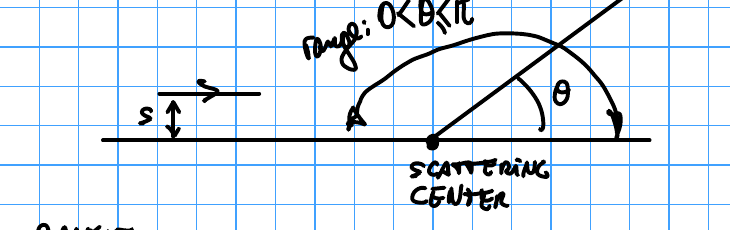
\includegraphics[width=0.55\textwidth]{figures/fig_scatter_center.png}
  \caption{Scattering-center geometry: a particle with impact parameter
  between $s$ and $s+ds$, incident along the horizontal line, is deflected by
  angle $\theta$ at the scattering center.}
  \label{fig:scatter-center}
\end{figure}

With $\sigma(\theta) = \tfrac14(ZZ'e^2/2E)^2\csc^4(\theta/2)$ and
$d\Omega = 2\pi\sin\theta\,d\theta = 4\pi\sin(\theta/2)\cos(\theta/2)\,d\theta$,
\[
  \sigma_T = \frac14\left(\frac{ZZ'e^2}{2E}\right)^2 \cdot 4\pi
  \int_0^\pi \frac{\sin(\theta/2)\cos(\theta/2)}{\sin^4(\theta/2)}\,d\theta
  = \pi\left(\frac{ZZ'e^2}{2E}\right)^2
  \int_0^\pi \frac{\cos(\theta/2)}{\sin^3(\theta/2)}\,d\theta
  \sim \int_0 \frac{d\theta}{(\theta/2)^3},
\]
which is \textbf{strongly divergent} as $\theta\to0$: classically,
$\sigma_T = +\infty$ for any long-range potential; quantum mechanically,
$\sigma_T=+\infty$ as well for potentials $V(r)$ that do not decay fast enough
as $r\to\infty$.

\begin{caveat}
In a dense, conducting material the bare Coulomb potential $V=-k/r$ is
replaced by the screened (``Yukawa'') potential
\[
  V^{\text{screen}}(r) = -\frac{k}{r}\,e^{-r/\lambda},
\]
which regularizes the divergence. In non-conducting materials
$V^{\text{screen}}(r)$ may take a different functional form, but will still
vanish much faster than $1/r$ as $r\to\infty$.
\end{caveat}

\section{The Hamiltonian and Hamilton's Equations of Motion}

We now turn to a different topic, which opens the course's Chapter~8
immediately following the scattering material of Sections~1--3 in the same
lecture: rather than continuing with the Lagrangian description
$L(q,\dot q,t)$ used implicitly above, we develop an equivalent formulation
in terms of the generalized coordinates and their conjugate momenta,
$(q,p,t)$. Starting from the Lagrangian $L = T - V = L(q_1,\dots,q_n,\dot q_1,\dots,\dot q_n,t)$
and the Euler--Lagrange equations
\[
  0 = \frac{d}{dt}\left(\frac{\partial L}{\partial \dot q_i}\right) - \frac{\partial L}{\partial q_i},
  \qquad p_i \equiv \frac{\partial L}{\partial \dot q_i}\bigg|_{q_j,\dot q_j},
\]

\begin{remark}[Midterm remark --- an invalid claim]
In plane polar coordinates it is tempting to write
$\partial L/\partial\dot\theta = p_\theta = \ell_z$ and conclude
$L = L(r,\dot r, p_\theta)$, i.e.\ to substitute the canonical momentum
$p_\theta$ directly back into the Lagrangian in place of $\dot\theta$. This
step is \textbf{invalid}: the Lagrangian is a function of the generalized
coordinates and \emph{velocities}, $L=L(q,\dot q,t)$; replacing $\dot q$ by its
conjugate momentum $p$ changes the independent variables and is precisely the
Legendre transformation carried out below to pass from $L$ to $H$ --- it
cannot be done term-by-term inside $L$ itself. Consequently the
crossed-out ``$\Rightarrow$ Lagrange Eqn.'' that follows in the original
notes is equally invalid: substituting the ill-defined $L(r,\dot r,p_\theta)$
into the Euler--Lagrange equation would silently discard the
$r$-dependence hidden inside $p_\theta = mr^2\dot\theta$. (Marked as crossed
out in the original notes as a caution against this common exam error.)
\end{remark}

\subsection{The Legendre Transformation}

The passage from $L(q,\dot q,t)$ to a new function of $(q,p,t)$ is an instance
of the general Legendre transformation. For $f(x,y)$ with
$df = \dfrac{\partial f}{\partial x}dx + \dfrac{\partial f}{\partial y}dy \equiv u\,dx + v\,dy$,
define $g = f - ux$; then
\[
  dg = df - d(ux) = u\,dx + v\,dy - u\,dx - x\,du = -x\,du + v\,dy,
\]
so $g = g(u,y)$: the transformation trades the variable $x$ for the
conjugate variable $u = \partial f/\partial x$.

\begin{remark}[Thermodynamic analogy]
The same transformation appears in thermodynamics. With the first law
$dU = \delta Q + \delta W = T\,dS - p\,dV$ (fluid at fixed particle number $N$),
$U=U(S,V)$ is the internal energy. To use $(T,V)$ as independent variables
instead, define the Helmholtz free energy $A = U - TS$:
\[
  dA = dU - d(TS) = (T\,dS - p\,dV) - T\,dS - S\,dT = -S\,dT - p\,dV
  \ \Rightarrow\ A = A(T,V),
\]
exactly the Legendre transform $g=f-ux$ with $(x,u)\to(S,T)$.
\end{remark}

\subsection{From the Lagrangian to the Hamiltonian}

Apply the Legendre transform to $L(q_1,\dots,q_n,\dot q_1,\dots,\dot q_n,t)$,
trading each $\dot q_i$ for its conjugate momentum $p_i = \partial L/\partial\dot q_i$.
Define
\[
  H \equiv -\Big(L - \sum_i p_i\dot q_i\Big) = \sum_i p_i \dot q_i - L.
\]
Then
\[
  dH = -dL + \sum_i d(p_i\dot q_i)
  = -\sum_i\left(\frac{\partial L}{\partial q_i}dq_i + \frac{\partial L}{\partial \dot q_i}d\dot q_i\right)
    - \frac{\partial L}{\partial t}dt
    + \sum_i \big(p_i\,d\dot q_i + \dot q_i\,dp_i\big),
\]
and since $\partial L/\partial \dot q_i = p_i$ the $d\dot q_i$ terms cancel:
\[
  dH = -\frac{\partial L}{\partial t}dt + \sum_i\left(\dot q_i\,dp_i - \frac{\partial L}{\partial q_i}dq_i\right)
  \ \Longrightarrow\ H = H(p_1,\dots,p_n,q_1,\dots,q_n,t).
\]
Using the Euler--Lagrange equation, $\partial L/\partial q_i = \dot p_i$, and
comparing the two expressions for $dH$ term by term gives \textbf{Hamilton's
canonical equations of motion}:
\begin{equation}
  \boxed{\ \frac{\partial H}{\partial p_i} = \dot q_i, \qquad
  \frac{\partial H}{\partial q_i} = -\frac{\partial L}{\partial q_i} = -\dot p_i, \qquad
  \frac{\partial H}{\partial t} = -\frac{\partial L}{\partial t}.\ }
  \label{eq:canonical}
\end{equation}

\end{document}
